\section{Research}
  I will now explore research done relating to the project specified. This will outline some design decisions that were made and link to other 
  sections of the report where they may be explored more. This section will explore parallelism and thread safety focusing on data stores as well as 
  CI/CD, it's pros and cons when deploying to live systems and how we as a team worked around it.

  % \subsection{Microservices and Cloud Computing}

  % IBM hows it being used - \url{https://www.ibm.com/downloads/cas/OQG4AJAM}
  % Pros and cons - \url{https://cdn.nrf.com/sites/default/files/2021-03/Microservices%20%20for%20Retail%20White%20Paper_The%20Good%2C%20The%20Bad%2C%20and%20The%20Better_JBS%20Custom%20Solutions.pdf}
  % adoption 2020 - \url{https://www.oreilly.com/radar/microservices-adoption-in-2020/}
  % Types of AWS services - \url{https://cdn2.hubspot.net/hubfs/1629777/A%20Comprehensive%20Guide%20on%20AWS%20as%20SaaS_IaaS_and_PaaS.pdf}
  % Types of cloud computing - \url{https://www.ibm.com/topics/cloud-computing}
  % 'Virutalisation is key for cloud computing' - \url{https://mooreks.co.uk/wp-content/uploads/2016/04/VirtualisationTheFussTheBuzzandtheAuditPlan.pdf}

  \subsection{Storage Solutions and Parallelism}
  \label{sec:storageSolutions}

  Currently the schedule pipeline consists of two components, the ingester, followed by the schedule generator. The first part of this pipeline is
  parallelised, multiple lambdas can be ran at the same time to insert data into the redis. This is a harder task for the schedule generator to do,
  as it needs update a list of linked schedules to an episode in the redis store. This data can be edited through multiple streams, both the schedule
  catalogue pipelines, meaning the array could easily become incorrect/polluted. Sharing memory in a threaded/parallelised system is a well known 
  challenge and you need to know when it's safe to update/edit this memories value (https://homes.cs.washington.edu/~djg/teachingMaterials/spac/sophomoricParallelismAndConcurrency.pdf).
  This is also known as being thread safe which can be described as \textit{'different threads can access the same resources without exposing erroneous 
  behavior or producing unpredictable results'} (Ugarte, A, 2024).

  \begin{figure}[H]
    \centering
    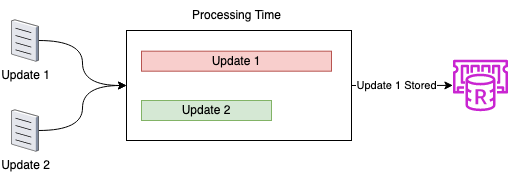
\includegraphics[width=6cm]{assets/raceCondition.drawio.png}
    \caption{Diagram showing how a broadcast list of an episode can become incorrect/polluted.}
    \label{fig:raceCondition}
  \end{figure}

  \subsubsection{Redis and Elasticache}
  We use amazons Elasticache (Amazon Web Services, 2024f) for our redis (REmote DIctionary Server) solution as it stores data in memory, which makes it 
  really quick to retrieve stored data (IBM, 2024). This is vital for us as we store large documents that need to be retrieved and sent to partners on 
  an API request. Redis is single-threaded but supports concurrency, \textit{'when at least two threads are making progress'} (Oracle Corporation, 2010) 
  which is not the same as parallelism, \textit{'when at least two threads are executing simultaneously'} (Oracle Corporation, 2010).

  \begin{figure}[H]
    \centering
    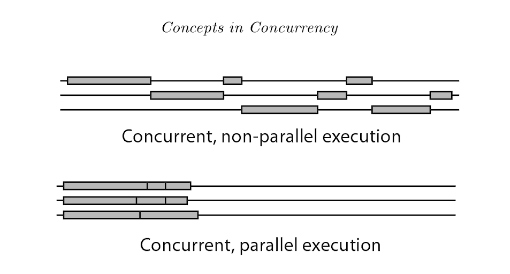
\includegraphics[width=8cm]{assets/concurrecnyVsParallelism.jpg}
    \caption{Difference between concurrency and parallelism. \url{https://books.google.ie/books/about/Introduction_to_Concurrency_in_Programmi.html?id=J5-ckoCgc3IC&redir_esc=y}}
    \label{fig:concurrecnyVsParallelism}
  \end{figure}

  This concurrency allows redis to support multiple requests at once, but it cannot do multiple operations at once; although more recent versions are allowing
  some safely threaded operations such as deleting records (Redis Ltd, 2024a). It also supports batch uploading and blocking commands, however these also 
  don't help keep the data thread-safe.

  \begin{itemize}
    \item \textbf{Pipelining} - Pipelining sends a block of commands at once, however does not guarantee that commands sent are done in sequence 
    (Redis Ltd, 2024b).
    \begin{figure}[H]
      \centering
      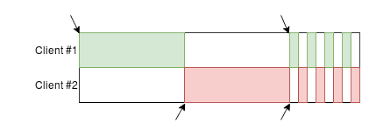
\includegraphics[width=8cm]{assets/pipelineOrdering.png}
      \caption{How redis pipelines don't guarantee sequential execution (Eyng, R, 2019).}
      \label{fig:pipelineOrdering}
    \end{figure}
    \item \textbf{Transactions} - Transactions are very similar to pipelines, however guarantee that the transactions commands are not interrupted by another
    clients requests and are therefore executed in sequence (Redis Ltd, 2024c).
    \item \textbf{Blocking Actions} - Blocking actions stop the current client from executing commands until the blocking action is complete. However other 
    clients can still send requests to the server whilst this client is blocked (Redis Ltd, 2024d). 
  \end{itemize}

  The options above still allow the previous race condition to occur, as instances of the schedule generator may vary in processing time and therefore the 
  time of writing to the redis cannot be guaranteed to be in order of the events.

  \subsubsection{How thread-safety can be achieved}
  When researching and spiking (Visual Paradigm, 2024) the project, other technologies were found that could help offer thread safety whilst parallelising
  the schedule generator. These were types of store/database locking mechanisms.

  \begin{itemize}
    \item \textbf{Pessimistic Locking} - This method \textit{'assumes that access to shared memory will be contended'} (Weston, T, 2011) and
    acquires a lock on the data to be edited. Any other client/connection attempting to edit this data must wait until this lock is released to update
    the data (Thornton, G, 2001). This can lead to issues such as deadlock which is when two clients are both awaiting on another clients lock to 
    be released. This can end up with both clients being stuck in a endless cycle of waiting for each other (Thornton, G, 2001; Apache Software Foundation, 2013).

    \begin{figure}[H]
      \centering
      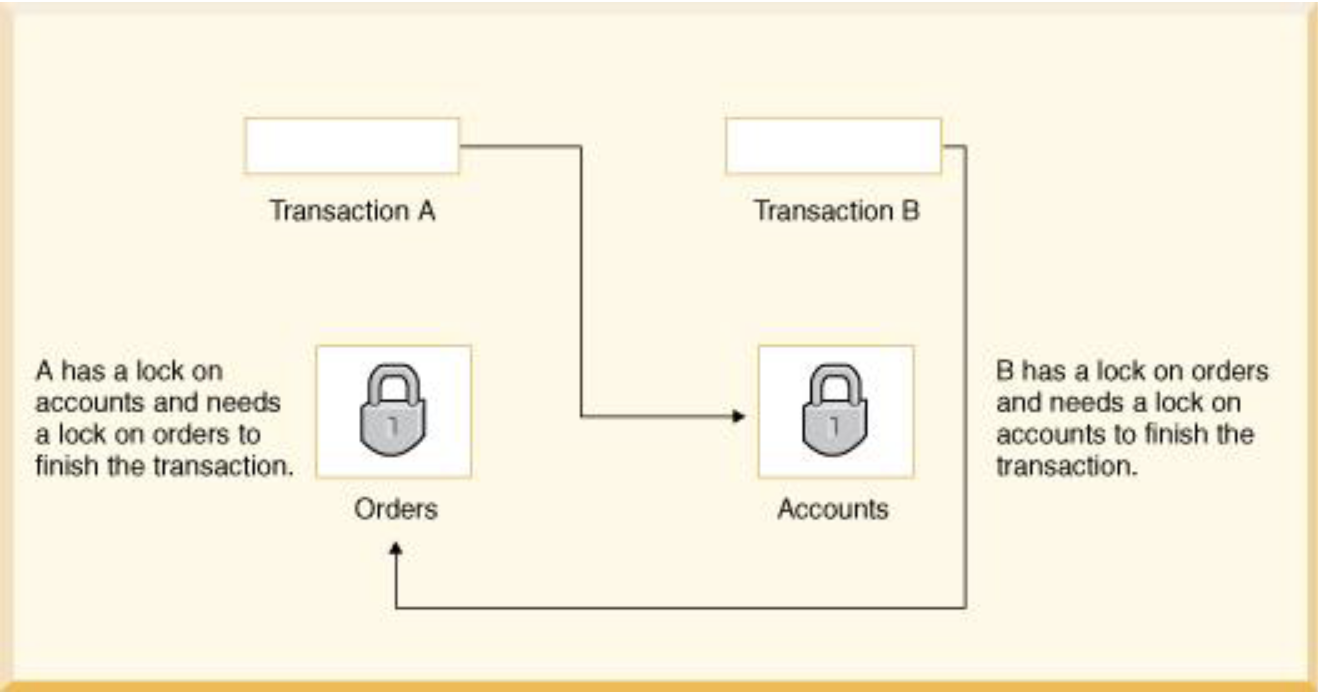
\includegraphics[width=8cm]{assets/deadlock.png}
      \caption{Example of a deadlock scenario (Apache Software Foundation, 2013).}
      \label{fig:deadlock}
    \end{figure}

    There is also a situation where a client locks a piece of data and for one reason or another halts, this would cause needless delay, when a timeout is 
    specified, if a timeout is not specified then this object would be locked from changes indefinitely (Thornton, G, 2001).

    \item \textbf{Optimistic Locking} - This method \textit{'relies on end-of-transaction validation'} (Graefe, G, 2016). Unlike its counterpart
    (pessimistic locking) it does not lock the record that is being updated. Instead before the new data is written, the original data is checked against 
    the current data stored (Thornton, G, 2001). If this data doesn't match then a change has occurred during processing and the new data to be written 
    must be re-calculated with the new changes.

    \begin{figure}[H]
      \centering
      \includegraphics[width=6cm]{diagrams/sequence/Optimistic Locking.png}
      \includegraphics[width=6cm, height=6cm]{diagrams/activity/Optimistic Locking.png}
      \caption{Sequence and activity diagrams outlining logic of optimistic locking.}
      \label{fig:optimisticLocking}
    \end{figure}

    This above logic could be implemented into our redis solution. It would require either a total comparison of the object or a simple \textit{version}
    field that specifies when the object has changed.
  \end{itemize}

  During this investigation DynamoDB (Amazon Web Services, 2024e) was highlighted as a potential option due to it supporting optimistic
  locking. The final decision was to not use it however and stick with the current solution as there was a want to get the project started to keep 
  up with our roadmap and not further investigate this option. There was also more unknowns with this technology as we had never used it before.
  I will discuss a solution using DynamoDB in the \hyperref[sec:future]{\textbf{Future Work}} section of this report.
   
  \subsection{CI/CD and it's challenges}

  Discussion on agile somewhere in here.

  Draw parallels to disaster recovery replication and measures.

  Deploying to Live systems -\url{https://core.ac.uk/download/pdf/226768285.pdf}
  Extra layer of threat - \url{https://media.defense.gov/2023/Jun/28/2003249466/-1/-1/0/CSI_DEFENDING_CI_CD_ENVIRONMENTS.PDF}
  CI/CD more commits but more issues - \url{https://arxiv.org/pdf/2303.16393.pdf}
  Good to use CI/CD in critical systems - \url{https://files.techmahindra.com/static/img/pdf/devsecops-continuous-testing-adoption-in-safety-critical-software.pdf}
  Cost of bugs - \url{https://www.testim.io/wp-content/uploads/2019/11/CI_CD-The-Solution-to-High-Cost-Quality_Sep-2018.pdf - This might be shit}
  Devops survey - \url{https://about.gitlab.com/developer-survey/previous/2022/}
  Cost of errors (use CI/CD to stop) - \url{https://raygun.com/blog/cost-of-software-errors/#cost}

  Tech debt definition - \url{https://www.productplan.com/glossary/technical-debt/}
  Technical debt - \url{http://jultika.oulu.fi/files/nbnfi-fe201902185288.pdf}

\newpage